%% ============================================================================
%% Sem-GeoDF — IEEE Access manuscript (official ieeeaccess.cls)
%% Template assets: ../template/  (see ../template/SOURCE.md)
%% Regenerate tables/figures:
%%   python3 scripts/make_sem_geodf_paper_assets.py \
%%     --root results/sem_geodf_ablation/paper_postfix --out paper/sem_geodf
%% Compile from this directory:
%%   tectonic -X compile main.tex
%% ============================================================================
\documentclass{ieeeaccess}

\usepackage{cite}
\usepackage{amsmath,amssymb,amsfonts}
\usepackage{algorithm}
\usepackage{algpseudocode}
\usepackage{graphicx}
\usepackage{textcomp}
\usepackage{booktabs}
\usepackage{multirow}
\usepackage{array}
\usepackage{url}
\usepackage{bm}
\usepackage{xcolor}
% hyperref is loaded by ieeeaccess.cls when needed; avoid double-load

\graphicspath{{../figures/}}
% Auto-generated by scripts/make_sem_geodf_paper_assets.py. Do not edit by hand.
\newcommand{\PaperResultRoot}{results/sem\_geodf\_ablation/paper\_postfix}
\newcommand{\PaperNViode}{3}
\newcommand{\PaperNEuroc}{\mbox{1--2}}
\newcommand{\PaperNTrials}{3}

\newcommand{\HoldoutBetter}{6}
\newcommand{\HoldoutSimilar}{0}
\newcommand{\HoldoutWorse}{2}

\newcommand{\DeltaCityNightHigh}{-56.9\%}
\newcommand{\DeltaParkingHigh}{-38.2\%}
\newcommand{\DeltaCityNightMid}{-38.8\%}
\newcommand{\DeltaParkingMid}{-52.0\%}

% Paired w_i ATE ablation macros (filled by make_sem_geodf_paper_assets.py once
% sem_geodf_noweight runs exist). Until then the manuscript reports the weight
% mechanism table rather than paired ATE deltas.
\newcommand{\AblationNCells}{--}
\newcommand{\AblationMeanWOff}{--}
\newcommand{\AblationMeanWOn}{--}
\newcommand{\AblationDeltaMean}{pending}
\newcommand{\AblationWeightBetter}{--}
\newcommand{\AblationWeightSimilar}{--}
\newcommand{\AblationWeightWorse}{--}


\begin{document}
\history{Date of publication xxxx 00, 0000, date of current version xxxx 00, 0000.}
\doi{10.1109/ACCESS.2026.DOI}

\title{Sem-GeoDF: Adaptive Gated Union of Semantic and Geometric Dynamic Feature Rejection for Stereo-Inertial Visual Odometry}

\author{\uppercase{Anonymous Author}\authorrefmark{1}}

\address[1]{Affiliation withheld pending author list finalization (IEEE Access submission draft).}

\tfootnote{Manuscript prepared with the IEEE Access \texttt{ieeeaccess} class. Code and configs will be released upon acceptance.}

\markboth
{Anonymous Author: Sem-GeoDF for Stereo-Inertial VIO}
{Anonymous Author: Sem-GeoDF for Stereo-Inertial VIO}

\corresp{Corresponding author: Anonymous Author (e-mail: anonymous@example.com).}

\begin{abstract}
Dynamic objects break the static-scene assumption used by feature-based stereo-inertial visual odometry (VIO).
Semantic segmentation masks can suppress movers but often over-reject useful structure in static scenes, whereas geometry-only epipolar filters need no training labels yet may fail when movers dominate the image.
This paper presents \textbf{Sem-GeoDF}, an engineering fusion module for stereo-inertial VINS-Fusion that combines a non-blocking YOLO dynamic mask with GeoDF-Adaptive epipolar rejection through an \emph{adaptive gated union} (logical OR), not intersection.
Each branch keeps its own scene gate; candidates are merged under a shared reject-ratio budget; and a three-state online policy (static-safe / dynamic-assist / strong-dynamic) modulates soft masking, hard cull, and adaptive backend residual weights \(w_i\in[w_{\min},1]\).
The policy uses only online signals---burst ratio, strong semantic EMA, and a Dice agreement score with an explicit minimum-support requirement on raw GeoDF candidates---and never reads dataset labels, ground truth, or hold-out metrics. Hard rejection additionally requires healthy experts, observable camera motion and sufficient feature redundancy, so deletion is gated by a per-track lifecycle rather than by evidence alone.
Under a fair \(1.0\times\) bag-rate protocol with thresholds tuned on VIODE \texttt{city\_day} only, Sem-GeoDF improves high-dynamic hold-out scenes versus GeoDF-Adaptive (e.g., city\_night/\(3\_high\)~\DeltaCityNightHigh, parking\_lot/\(3\_high\)~\DeltaParkingHigh) while reducing static-scene regression relative to always-on semantic masking (SAD-Sem).
We do not claim per-cell superiority over SAD-Sem on mean ATE; the contribution is spectrum robustness, protocol hygiene, and a reproducible evaluation on VIODE (\(N=\PaperNViode\) trials per cell) and EuRoC as a static-scene safety check (\(N=\PaperNEuroc\) trials per cell). The numerical results reported here predate the correctness and fairness fixes described in Sec.~\ref{sec:status} and are being regenerated; the method description and its test-enforced correspondence to the implementation are current.
On the eight dynamic hold-out scenes, Sem-GeoDF is better than GeoDF-Adaptive on \HoldoutBetter{} and worse on \HoldoutWorse{} under a \(\pm3\%\) band.
\end{abstract}

\begin{keywords}
Dynamic feature rejection, stereo-inertial odometry, semantic segmentation, sensor fusion, visual-inertial SLAM, residual weighting, YOLO
\end{keywords}

\titlepgskip=-15pt

\maketitle

\section{Introduction}
\label{sec:introduction}
\IEEEPARstart{S}{tereo}-inertial visual odometry (VIO) estimates ego-motion by fusing camera tracks with inertial measurements and is a core building block for mobile robots, drones, and AR navigation~\cite{qin2018vins,qin2019vinsfusion}.
Most feature-based front-ends assume that the majority of tracked points lie on a rigid static scene.
That assumption fails in traffic-like environments: moving vehicles inject inconsistent image motion into the visual residual and inflate absolute trajectory error (ATE), as stressed by dynamic benchmarks such as VIODE~\cite{minoda2021viode}.

Two complementary remedy families are widely used.
\emph{Semantic} methods remove features that fall on detector or instance/segmentation masks~\cite{bescos2018dynaslam,yu2018dsslam,song2022dynavins}.
They are effective when the model fires correctly, but false positives can strip static structure, and accuracy becomes coupled to model domain, class taxonomy, and compute budget.
\emph{Geometric} methods reject tracks that violate multi-view rigidity, typically via epipolar Sampson tests and robust fundamental-matrix estimation~\cite{hartley2003multiple}.
They require no semantic training data, yet a fundamental matrix estimated from a mover-dominated image can itself become unreliable.

This paper addresses a practical systems question for stereo-inertial VINS:
\emph{How can semantic and geometric experts be combined online, without oracle scene labels, so that static safety stays close to geometry-only behavior while high-dynamic accuracy exceeds geometry alone?}
We propose \textbf{Sem-GeoDF}, a policy-gated \emph{union} (OR) of YOLO and GeoDF-Adaptive candidates under one shared reject-ratio guard, with optional adaptive backend residual weighting for suspicious survivors.

\paragraph{Contributions.}
\begin{enumerate}
\item An online adaptive gated-union front-end for stereo-inertial VINS that ORs semantic and GeoDF dynamic candidates with a shared ratio/min-feature guard and non-blocking mask synchronization.
\item A label-free three-state policy (static-safe / dynamic-assist / strong-dynamic) driven by burst/strong EMA and a support-guarded Dice agreement score on \emph{raw} GeoDF candidates, with holds expressed as durations on the sensor clock rather than frame counts.
\item Adaptive backend residual weights \(w_i\) with Ceres \(\sqrt{w_i}\) scaling, computed only from online semantic/geometric evidence and per-id recovery.
\item A reproducible evaluation: fair \(1.0\times\) bag rate, thresholds selected on \texttt{city\_day} only, hold-out \texttt{city\_night}/\texttt{parking\_lot} (\(N=\PaperNViode\)) and an EuRoC static check (\(N=\PaperNEuroc\) trials per cell), with a four-method matrix switched by \texttt{METHODS}. All reported tables are regenerated directly from run artifacts by one script, with the per-cell trial count printed in every cell.
\item A correctness and fairness layer that makes the evaluation checkable rather than asserted: all methods are generated from one common backbone with a machine-checked ownership allowlist; a stereo physical validity contract is shared by the backend and the geometric branch; the fundamental matrix is tested for degeneracy before it may authorise a deletion; failure detection is structured and recorded; and no publication asset can be produced from a run tree that has not passed an expected-matrix gate.
\item Honest positioning: we emphasize spectrum robustness and static safety rather than claiming universal best ATE against semantic-only baselines, and we state explicitly which evidence is still outstanding (Sec.~\ref{sec:status}).
\end{enumerate}

\section{Related Work}
\label{sec:related}
\subsection{Dynamic visual and visual-inertial SLAM}
Handling dynamic scenes has been a long-standing goal for feature-based SLAM~\cite{cadena2016survey}.
DynaSLAM and DS-SLAM combine geometric motion cues with semantic segmentation for visual SLAM~\cite{bescos2018dynaslam,yu2018dsslam}, and DynaSLAM~II tightly couples multi-object tracking with the estimator~\cite{bescos2021dynaslam2}.
More recent semantic-geometric systems refine this idea: RDS-SLAM removes the tracking-thread stall of semantic masks~\cite{zhang2020rdsslam}, CFP-SLAM uses a coarse-to-fine dynamic-probability model~\cite{hu2023cfpslam}, Crowd-SLAM targets crowded scenes with detection~\cite{soares2021crowd}, and DytanVO jointly refines odometry and motion segmentation~\cite{shen2023dytanvo}.
On the visual-inertial side, DynaVINS adds robust pose-graph factors for dynamic environments~\cite{song2022dynavins}, and Liu \emph{et al.}~\cite{liu2022dynamicvins} combine object detection with IMU for resource-restricted RGB-D robots.
Those full-stack systems are strong references and generally target either RGB-D or full SLAM back-ends.
Our scope is intentionally narrower and complementary: a drop-in stereo-inertial front-end module for VINS-Fusion with non-blocking mask synchronisation, an online label-free policy, optional backend residual weighting, and protocol hygiene (no label leakage into the online estimator). We describe the design as non-blocking rather than \emph{real-time}: a real-time claim requires end-to-end mask age and frame-drop rate to be measured and reported, which we do in Sec.~\ref{sec:runtime} rather than assert.
We do not claim to outperform these full stacks; we target a reproducible, honestly-scoped fusion component.

\subsection{Geometry-only dynamic feature rejection}
Epipolar geometry and Sampson residuals are classical tools~\cite{hartley2003multiple}.
Always-on geometric filters risk removing static structure during aggressive rotation or low parallax.
GeoDF-Adaptive introduces scene-aware activation with an auto-calibrated \(\rho_{\mathrm{on}}\) and track-level voting; Sem-GeoDF reuses this branch unchanged as the geometric expert.

\subsection{Semantic masking in VIO}
Real-time instance/segmentation networks such as YOLO~\cite{redmon2016yolo,jocher2023yolo} provide dynamic-object pixels at interactive rates.
Our SAD-Sem ablation applies semantic masking alone under the same fair bag rate and therefore isolates the benefit of fusion versus ``semantics always on.''

\subsection{How Sem-GeoDF differs}
Table~\ref{tab:diff} and Fig.~\ref{fig:fusion} contrast design choices.
AND fusion rejects only when both experts agree and can miss movers when one expert is silent.
Sequential cascades apply one filter after the other without a shared budget.
Sem-GeoDF uses policy-gated OR with a shared reject-ratio guard and a static-safe mode that disables semantic hard cull until online evidence escalates.

\begin{figure}[t]
\centering
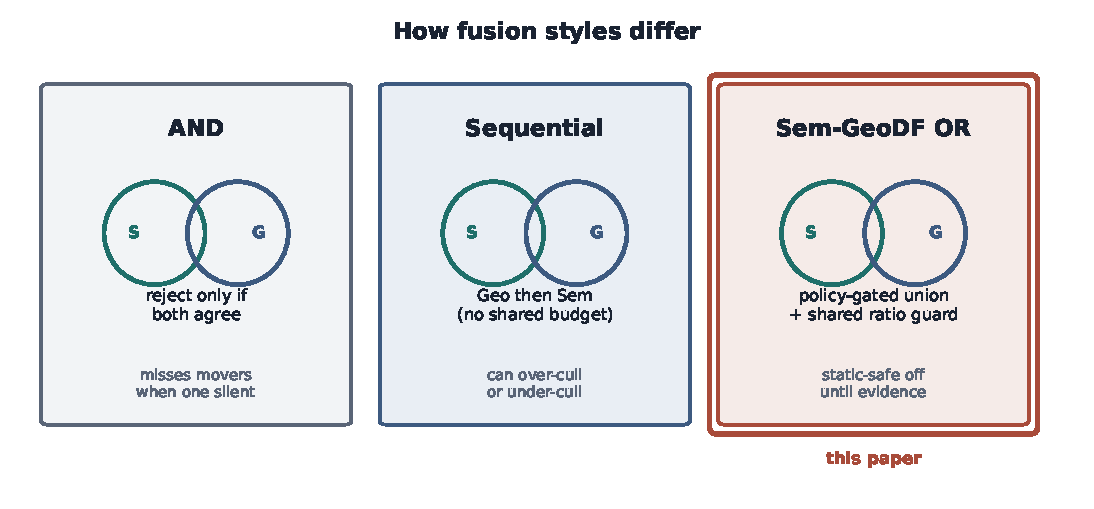
\includegraphics[width=\columnwidth]{fusion_compare_sem_geodf.pdf}
\caption{Conceptual contrast of fusion styles. Sem-GeoDF uses a policy-gated union (OR) with a shared reject budget rather than AND agreement or an unbudgeted sequential cascade.}
\label{fig:fusion}
\end{figure}

\begin{table}[t]
\centering
\caption{Conceptual design contrast among fusion styles.}
\label{tab:diff}
\setlength{\tabcolsep}{3.5pt}
\begin{tabular}{lccc}
\toprule
Aspect & AND & Sequential & Sem-GeoDF \\
\midrule
Reject if either expert fires & no & partial & yes (OR) \\
Shared reject-ratio budget & rare & no & yes \\
Static-safe semantic hard-cull off & rare & no & yes \\
Label-free online policy & varies & varies & yes \\
Adaptive backend residual weights & rare & rare & yes (optional) \\
\bottomrule
\end{tabular}
\end{table}

\section{Method}
\label{sec:method}
\subsection{System overview}
Fig.~\ref{fig:overview} gives a full-system view of Sem-GeoDF inside stereo-inertial VINS-Fusion; Fig.~\ref{fig:pipeline} compresses the same front-end into a per-frame flow.
Camera images feed YOLO asynchronously (\(\texttt{sem\_block\_on\_mask}{=}0\)).
If the latest mask is older than \(\texttt{sem\_mask\_max\_age\_ms}\), the semantic branch is disabled for that frame (fail-open to geometry).
Previous tracks feed GeoDF-Adaptive.
Confirmed semantic and geometric candidates are unioned, clipped by \(\texttt{geodf\_max\_reject\_ratio}\) and a minimum feature count, then optionally enter backend optimization with residual weights \(w_i\).

\paragraph{Design principles.}
\begin{itemize}
\item \emph{No oracle leakage:} the estimator never reads VIODE level, ground truth, ATE/RPE, or summary files.
\item \emph{Fail-open semantics:} missing/stale masks never stall VINS.
\item \emph{Union under a budget:} OR fusion cannot wipe the track set.
\item \emph{Train/hold-out hygiene:} policy thresholds are frozen from \texttt{city\_day} before inspecting hold-out ATE.
\end{itemize}

\begin{figure*}[t]
\centering
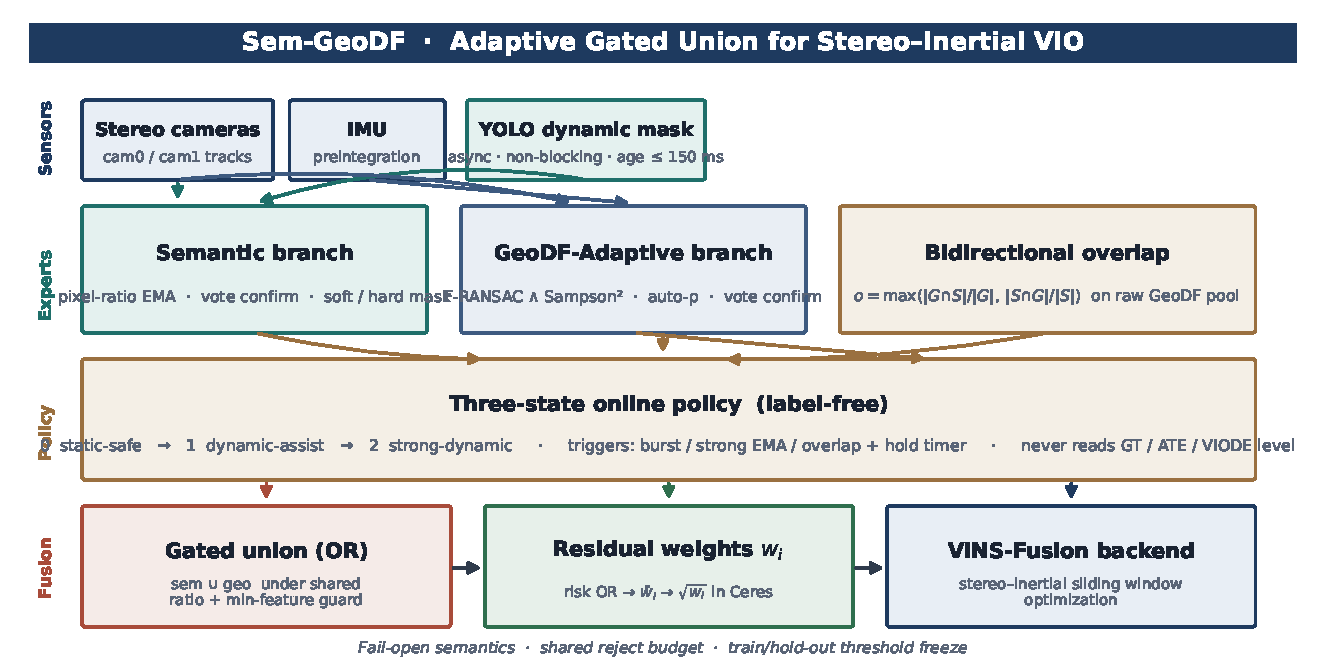
\includegraphics[width=0.98\textwidth]{system_overview_sem_geodf.pdf}
\caption{Sem-GeoDF system overview. Sensors feed a semantic expert (YOLO) and a GeoDF-Adaptive geometric expert; bidirectional overlap and a label-free three-state policy gate a shared OR union, optional residual weights \(w_i\), and the VINS-Fusion backend.}
\label{fig:overview}
\end{figure*}

\begin{figure}[t]
\centering
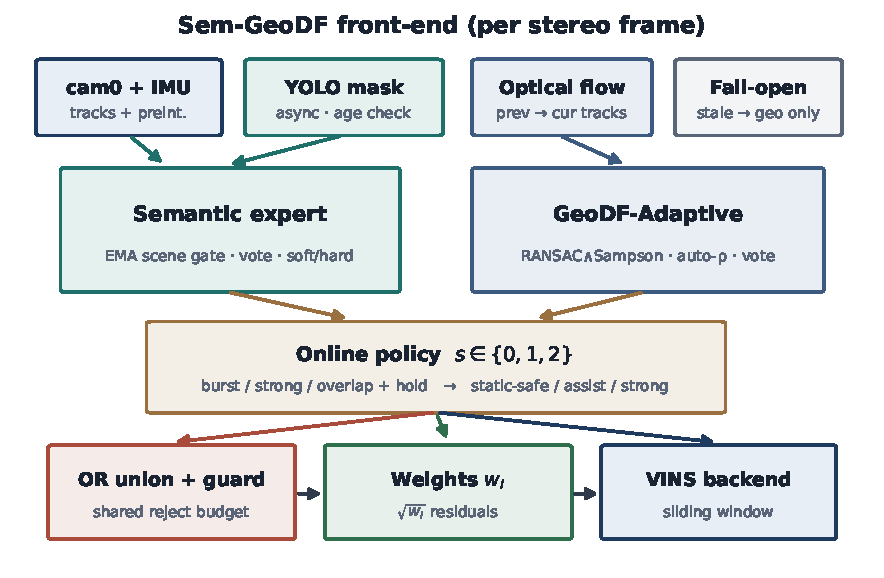
\includegraphics[width=\columnwidth]{pipeline_sem_geodf.pdf}
\caption{Per-frame Sem-GeoDF front-end: fail-open mask sync, dual experts, online policy, gated OR under a shared reject budget, and \(\sqrt{w_i}\) residual weighting into VINS.}
\label{fig:pipeline}
\end{figure}

\subsection{Geometric branch (GeoDF-Adaptive)}
A temporal fundamental matrix is estimated from track correspondences.
RANSAC inliers/outliers and Sampson residuals form a dual gate; tracks accumulate votes over \(\texttt{geodf\_vote\_frames}\).
Scene activation uses an EMA of the epipolar outlier ratio with hysteresis around an auto-calibrated \(\rho_{\mathrm{on}}\).
Confirmed geometric candidates enter the shared reject set whenever GeoDF is armed.

\subsection{Semantic branch}
\label{sec:masksync}
YOLO produces a dynamic-class mask on cam0.
Per-track hits are vote-confirmed over \(\texttt{sem\_vote\_frames}\).
A semantic scene gate tracks an EMA of the dynamic pixel ratio with hysteresis.
Soft masking of \emph{new} features and hard cull of \emph{existing} tracks are policy-dependent (Sec.~\ref{sec:policy}).

\subsection{Expert agreement with minimum support}
\label{sec:overlap}
An earlier implementation computed overlap only on GeoDF \emph{confirmed} tracks while \(\texttt{frame\_active}\), which empirically produced \(0\%\) overlap triggers even when both branches fired.
Sem-GeoDF therefore measures agreement on the raw GeoDF candidate pool \(G\) (fallback to confirmed if empty) and the semantic-raw set \(S\) (Fig.~\ref{fig:overlap}).

A directed maximum, \(o=\max(|G\cap S|/|G|,\,|S\cap G|/|S|)\), was used initially, but it is not a safe agreement measure: two two-element sets sharing a single track score \(o{=}0.5\) and clear a \(0.35\) threshold on coincidence alone. We use the symmetric S{\o}rensen--Dice coefficient
\begin{equation}
\label{eq:dice}
o_D=\frac{2\,|G\cap S|}{|G|+|S|},
\end{equation}
which cannot be dominated by the smaller set, together with an explicit \emph{minimum support} requirement
\begin{equation}
\label{eq:support}
|G|\ge n_G,\qquad |S|\ge n_S,\qquad |G\cap S|\ge n_I .
\end{equation}
When \eqref{eq:support} is not met the agreement signal is set to zero rather than passed to a threshold comparison, because a ratio computed from two or three tracks is not evidence. Optionally the score is scaled by a support confidence \(o_{\mathrm{sup}}=o_D\cdot\min(1,|G\cap S|/n_{\mathrm{sat}})\), which downweights small but qualifying intersections. The chosen metric is EMA-smoothed with coefficient \(\texttt{sem\_policy\_overlap\_ema}\).
Directional max, directional min, Dice, Jaccard and Dice-with-support are all implemented and selected by \(\texttt{sem\_policy\_overlap\_metric}\), so the choice is an ablation rather than an assumption (Table~\ref{tab:required_tables}).

\begin{figure}[t]
\centering
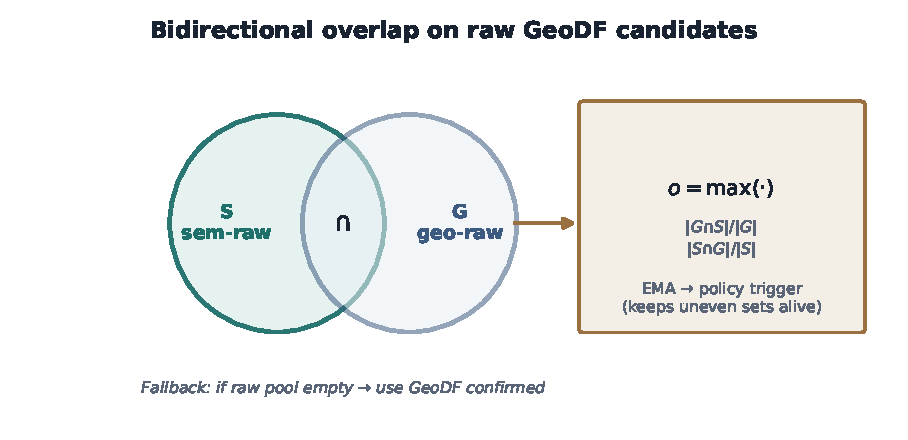
\includegraphics[width=0.92\columnwidth]{overlap_bidirectional.pdf}
\caption{Expert agreement on the raw GeoDF pool. Dice is symmetric, so the smaller candidate set cannot dominate the score, and the minimum-support requirement prevents a single shared track between two tiny sets from arming the policy.}
\label{fig:overlap}
\end{figure}

\subsection{Three-state adaptive policy}
\label{sec:policy}
Let the discrete state be \(s\in\{0,1,2\}\) (static-safe, dynamic-assist, strong-dynamic), as summarized in Fig.~\ref{fig:policy}.
Write \(r_t\) for the current-frame dynamic-pixel ratio, \(\bar{r}_t\) for its EMA, and \(\bar{o}_t\) for the overlap EMA of Sec.~\ref{sec:overlap}.
Escalation uses three online predicates:
\begin{align}
\mathrm{burst} &= [r_t \ge \tau_{\mathrm{burst}}], \\
\mathrm{strong} &= [\bar{r}_t \ge \tau_{\mathrm{strong}}], \\
\mathrm{overlap} &= [\bar{o}_t \ge \tau_{\mathrm{ov}} \;\wedge\; \eqref{eq:support}],
\end{align}
with defaults / train-selected values in Table~\ref{tab:params}.

\paragraph{The hold is a duration, not a frame count}
The hold was originally \(H\) frames (\(\texttt{sem\_policy\_hold\_frames}{=}180\)). A frame count is not a well-defined quantity: at \(10\)~Hz it is \(18\)~s, at \(30\)~Hz it is \(6\)~s, and it shortens further whenever frames are dropped, so the same configuration means different things on different sensors. The hold is now a duration on the \emph{sensor} clock (never wall-clock),
\begin{equation}
\label{eq:hold}
t^{\mathrm{hold}} \leftarrow \max\!\left(t^{\mathrm{hold}},\, t + \Delta_{\mathrm{assist}}\right),\qquad
\mathrm{hold\ active} = \left[\,t < t^{\mathrm{hold}}\,\right],
\end{equation}
with separate \(\Delta_{\mathrm{assist}}\) and \(\Delta_{\mathrm{strong}}\). A minimum dwell time prevents state chatter, and blocks only \emph{downgrades}: escalation is never delayed, because waiting is the unsafe direction when real dynamic content appears. A backwards timestamp (bag restart) resets the machine rather than leaving a hold armed for the remainder of the run.

\begin{itemize}
\item \(s{=}0\) (static-safe): soft-mask new features when the semantic scene is active; semantic hard cull off.
\item \(s{=}1\) (dynamic-assist): entered on burst, overlap, or an active hold; vote-confirmed semantic tracks enter the shared reject set when the semantic scene is active.
\item \(s{=}2\) (strong-dynamic): entered on strong EMA and/or assist plus usable raw geo evidence; full OR fusion armed under the same shared reject budget.
\end{itemize}
Final selected values are written to \texttt{selected\_params.yaml} from \texttt{city\_day} replay only (never from hold-out ATE).

\begin{figure}[t]
\centering
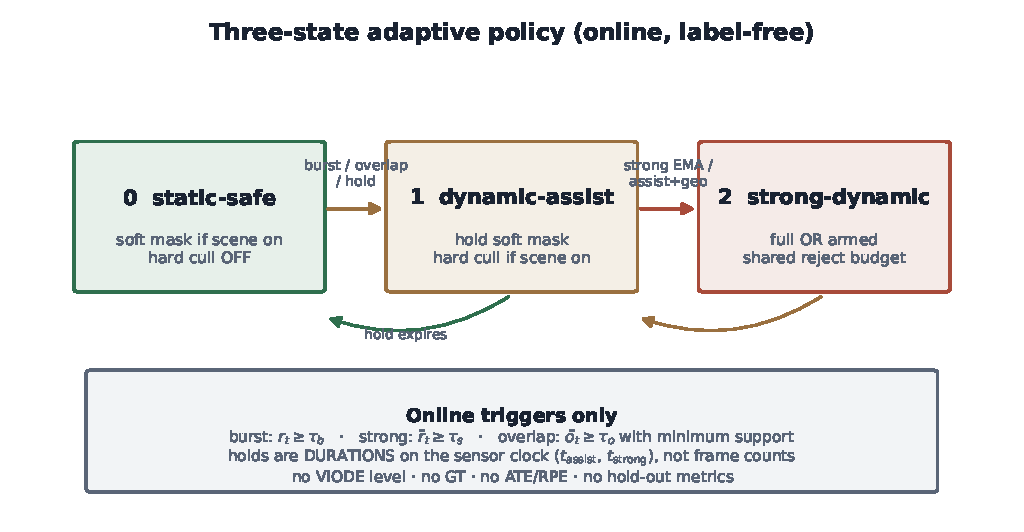
\includegraphics[width=\columnwidth]{policy_fsm_sem_geodf.pdf}
\caption{Three-state online policy. Escalation uses burst, strong semantic EMA, and bidirectional overlap only; the estimator never reads VIODE level, ground truth, or trajectory metrics.}
\label{fig:policy}
\end{figure}

\begin{table}[t]
\centering
\caption{Key Sem-GeoDF parameters (defaults / train-selected).}
\label{tab:params}
\begin{tabular}{lc}
\toprule
Parameter & Value \\
\midrule
\(\texttt{sem\_vote\_frames}\) / \(\texttt{geodf\_vote\_frames}\) & 2 / 2 \\
\(\texttt{sem\_policy\_burst\_ratio}\) & 0.18 \\
\(\texttt{sem\_policy\_strong\_ratio}\) & 0.18 (selected) \\
\(\texttt{sem\_policy\_hold\_frames}\) & 180 (selected) \\
\(\texttt{sem\_policy\_overlap\_ratio}\) & 0.35 \\
\(\texttt{geodf\_max\_reject\_ratio}\) & 0.40 \\
\(\texttt{sem\_mask\_max\_age\_ms}\) & 150 \\
\(\texttt{sem\_geodf\_backend\_weight}\) & 1 (enabled) \\
\(\texttt{sem\_geodf\_backend\_min\_weight}\) & 0.25 \\
\(\texttt{sem\_geodf\_backend\_recovery}\) & 0.20 \\
\bottomrule
\end{tabular}
\end{table}

\subsection{Health, observability and per-track lifecycle}
\label{sec:health}
Neither expert is trustworthy unconditionally, so evidence is not allowed to act directly. Three health scores in \([0,1]\) are measured first, and only then does a policy decide what may be done.

\emph{Semantic health} \(h_{\mathrm{sem}}\) falls with mask staleness (using the mask's own source timestamp, Sec.~\ref{sec:masksync}) and with mask \emph{saturation}: a mask that labels most of the frame dynamic is far more often a segmentation failure than a scene in which everything moves, so it must not be permitted to delete features.

\emph{Geometric health} \(h_{\mathrm{geo}}\) comes from an explicit degeneracy test on the fundamental matrix, rather than from \(F\) merely being non-empty. \(F\) estimated during near-pure rotation, at low parallax, from correspondences clustered in one image region, from weak RANSAC support, or from a mover-dominated frame is not empty --- it is confidently wrong, and hard-rejecting static structure on it is precisely the failure mode this work claims to avoid. We therefore require a minimum median parallax, a minimum grid occupancy, a bounded residual-spread condition number, and minimum RANSAC inlier count and ratio. Low parallax and an ill-conditioned estimate mark the geometry \emph{degenerate} (no GeoDF decision at all); clustered features, weak support and mover dominance mark it \emph{weak} (down-weight only, and not admissible as strong two-expert agreement).

\emph{Observability health} \(h_{\mathrm{obs}}\) is the \emph{minimum} of normalized redundancy (track count), median parallax, and spatial spread. The minimum, not a mean: many features clustered in one corner do not make camera motion observable.

Each track then carries its own lifecycle,
\[
\textsc{Trusted}\to\textsc{Suspect}\to\textsc{DownWeighted}\to\textsc{Rejected},
\]
with \(\textsc{Suspect}/\textsc{DownWeighted}\to\textsc{Recovering}\to\textsc{Trusted}\) when evidence disappears and the track stays clean for a dwell time. Hard rejection is the only irreversible action, and a track may be deleted only when \emph{all} of the following hold:
\begin{equation}
\label{eq:reject-guard}
r_i \ge \tau_{\mathrm{rej}}
\;\wedge\;
\text{two-expert agreement}
\;\wedge\;
h_{\mathrm{sem}},h_{\mathrm{geo}} \text{ healthy}
\;\wedge\;
h_{\mathrm{obs}} \text{ healthy}
\;\wedge\;
N_{\mathrm{track}} \ge N_{\min},
\end{equation}
and a per-frame deletion allowance of \(N_{\mathrm{track}}-N_{\min}\) bounds how many tracks a single frame may remove. Without that allowance, evaluating \(N_{\mathrm{track}} \ge N_{\min}\) once per track lets a batch of simultaneous deletions overshoot the floor. Anything short of \eqref{eq:reject-guard} is a recoverable down-weight, and which guard blocked a deletion is logged so the behaviour is auditable rather than invisible.

This is the substantive difference from an OR fusion under a reject-ratio cap: what the method manages is a factor \emph{lifecycle} governed by evidence quality, redundancy and estimator observability.

\subsection{Stereo physical validity contract}
\label{sec:stereo}
A stereo match previously had to satisfy only optical flow plus a fixed left--right cycle tolerance. Nothing verified that it was physically possible, so a match with the wrong disparity direction or a negative triangulated depth could reach the stereo factor, depth initialisation, the right-camera geometric branch and the weight evidence.

Every left--right match now passes one contract before any consumer sees it: flow status and border validity; a left\(\to\)right\(\to\)left cycle bound; an epipolar residual against \(E=[\mathbf{t}]_\times R\) from the actual extrinsic; a disparity magnitude within \([d_{\min},d_{\max}]\); positive triangulated depth in \emph{both} cameras; and a bounded distance between the two rays at closest approach.

Crucially, the expected disparity \emph{direction} is derived per feature rather than hard-coded. For a ray \(\mathbf{x}_0\) in cam0 at inverse depth \(w=1/Z\), the cam1 projection is \(\pi(R\mathbf{x}_0 + w\mathbf{t})\), which starts at the point at infinity \(\pi(R\mathbf{x}_0)\) for \(w{=}0\) and moves along the epipolar line as \(w\) grows; a physically possible match lies on that side. This is exact for any rig geometry, so the same test is valid for left--right, right--left, vertical and verged rigs, whereas ``disparity must be positive'' is a calibration-specific assumption.

There is exactly one stereo matcher. The geometric branch reads only contract-validated observations instead of running a second optical flow of its own, which previously let its measurement of a track disagree with the measurement the backend factor used for the same track. Per-cause counters (wrong disparity sign, cycle, epipolar, negative depth, reprojection, range, border) are logged for every frame, so a published rejection rate is accountable.

\subsection{Failure detection}
\label{sec:failure}
A diverged run must be reported as failed, not emit a plausible-looking trajectory that then enters a table. The estimator evaluates, per frame and most-severe-first: non-finite state, solver failure, accelerometer- and gyroscope-bias divergence, translation and rotation jumps, and a \emph{sustained} run of low-feature frames (a single sparse frame is normal). The reason is structured (\textsc{NanState}, \textsc{SolverFailure}, \textsc{AccBiasDivergence}, \textsc{GyroBiasDivergence}, \textsc{TranslationJump}, \textsc{RotationJump}, \textsc{LowFeatureCount}) and written to the run manifest with its timestamp, so failures are counted rather than inferred.

\subsection{Adaptive backend residual weighting}
\label{sec:weight}
Hard rejection is not always possible: a shared ratio guard and minimum-feature constraints may keep suspicious tracks alive.
When \(\texttt{sem\_geodf\_backend\_weight}{=}1\), each surviving track \(i\) carries a residual weight \(w_i\in[w_{\min},1]\), broadcast to all of its observations and combined as the per-pair minimum across the two frames of a factor (Fig.~\ref{fig:weight}).
Every visual factor in Ceres multiplies both the residual \emph{and} all of its Jacobian blocks (including the time-offset term) by \(\sqrt{w_i}\), so the contribution is a genuine weighted least-squares term rather than an untracked post-hoc score.
The weight is thus a per-track confidence, not an independent per-observation noise model; we state this explicitly to avoid overclaiming.

\begin{figure}[t]
\centering
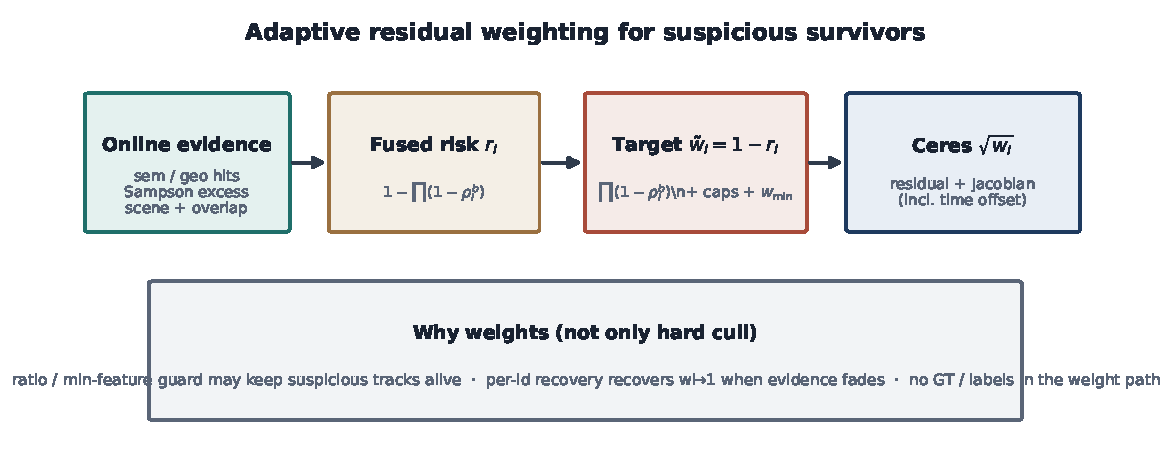
\includegraphics[width=\columnwidth]{backend_weight_flow.pdf}
\caption{Adaptive residual-weight path for tracks that survive the shared reject budget. Online semantic/geometric evidence forms a fused risk \(r_i\) by multiplicative (noisy-OR-inspired) fusion; the target weight is its inverse \(\tilde{w}_i{=}\mathrm{clip}(1{-}r_i,w_{\min},1)\), recovered per id, then applied as \(\sqrt{w_i}\) in Ceres.}
\label{fig:weight}
\end{figure}

From online evidence at the current frame we form three risk terms in \([0,1]\):
\begin{align}
\rho^{\mathrm{sem}}_i &= \mathbb{1}^{\mathrm{sem}}_i\,(1{-}w_{\mathrm{sem}})\,c^{\mathrm{sem}}_i, \\
\rho^{\mathrm{geo}}_i &= \mathbb{1}^{\mathrm{geo}}_i\,(1{-}w_{\mathrm{geo}})\,\max(c^{\mathrm{geo}},\,e_i), \\
\rho^{\mathrm{agr}}_i &= \mathbb{1}^{\mathrm{sem}}_i\mathbb{1}^{\mathrm{geo}}_i\,(1{-}w_{\mathrm{agr}})\,\max(\bar{o}_t,\,\min(c^{\mathrm{sem}}_i,\max(c^{\mathrm{geo}},e_i))),
\end{align}
where \(\mathbb{1}^{\mathrm{sem}}_i\) / \(\mathbb{1}^{\mathrm{geo}}_i\) flag semantic / GeoDF raw-or-confirmed hits, \(c^{\mathrm{sem}}\) / \(c^{\mathrm{geo}}\) are scene confidences from EMA+hysteresis (and policy state), and \(e_i\) is the normalized Sampson excess.
A multiplicative fusion (noisy-OR-inspired; we do \emph{not} assume the three evidence terms are independent, so we avoid calling it a probabilistic OR) combines them into a single \emph{fused risk}
\begin{equation}
\label{eq:fused-risk}
r_i = 1-\!\!\prod_{b\in\{\mathrm{sem},\mathrm{geo},\mathrm{agr}\}}\!\!\left(1-\rho^{b}_i\right),
\end{equation}
which is then mapped to a target weight by \emph{inverting} the risk,
\begin{equation}
\label{eq:target-weight}
\tilde{w}_i = \mathrm{clip}\!\left(1-r_i,\; w_{\min},\;1\right)
            = \mathrm{clip}\!\left(\prod_{b}\left(1-\rho^{b}_i\right),\; w_{\min},\;1\right),
\end{equation}
so that more dynamic evidence always yields a \emph{smaller} weight.
Afterwards \(\tilde{w}_i\) is capped by \(w_{\mathrm{sem}}\), \(w_{\mathrm{geo}}\), or \(w_{\mathrm{agr}}\) when the corresponding confirmation flags fire, and re-clipped to \([w_{\min},1]\).
Eqs.~\eqref{eq:fused-risk}--\eqref{eq:target-weight} are enforced against the implementation by the property test \texttt{PaperEquationMatchesImplementation}, together with the monotonicity property that raising any evidence confidence never raises \(\tilde{w}_i\).
Per-id recovery with rate \(\alpha_{\mathrm{rec}}\) raises \(w_i\) toward a higher target gradually so transient false positives do not permanently suppress a track:
\begin{equation}
w_i \leftarrow
\begin{cases}
w_i^{\mathrm{prev}}+\alpha_{\mathrm{rec}}(\tilde{w}_i-w_i^{\mathrm{prev}}) & \text{if }\tilde{w}_i>w_i^{\mathrm{prev}},\\
\tilde{w}_i & \text{otherwise.}
\end{cases}
\end{equation}
\paragraph{Consistency with marginalization}
Each observation's weight is frozen when its residual block is constructed (\(\sqrt{w_i}\) is a \texttt{const} member of the factor), so:
\begin{quote}
Recovery changes the weight of \emph{new} observations of the same track; residuals that have already been marginalized retain the weight they were created with.
\end{quote}
The marginalization factor therefore never reads a mutable global weight, and updating a track's current weight cannot retroactively alter a prior that has already been formed. This invariant is checked by \texttt{test\_marginalization\_weight\_freeze}.

Audit columns in \(\texttt{sem\_geodf\_stats.csv}\) separate the three quantities of Sec.~\ref{sec:weight}: \(\texttt{mean\_target\_weight\_pre\_guard}\) (mapping output), \(\texttt{mean\_applied\_weight\_post\_guard}\) and \(\texttt{min\_survivor\_weight}\) (after recovery, over tracks that survived the shared reject budget), plus \(\texttt{weighted\_candidates\_pre\_guard}\), \(\texttt{weighted\_survivors\_post\_guard}\) and \(\texttt{rejected\_weighted\_tracks}\) so that down-weighting is reported for survivors rather than for candidates.
Table~\ref{tab:ablation_weight} lists the defaults used in paper configs.

\begin{algorithm}[t]
\caption{Sem-GeoDF front-end step (per stereo frame)}
\label{alg:semgeodf}
\begin{algorithmic}[1]
\State Sync latest YOLO mask if age \(\le\) max age; else disable semantic branch
\State Update semantic EMA; run GeoDF-Adaptive \(\to\) raw/confirmed sets
\State Compute bidirectional overlap \(o\) on raw GeoDF pool; update policy \(s\)
\State \(R \gets\) GeoDF confirmed \(\cup\) (policy-gated semantic confirmed)
\State Apply shared ratio / min-feature guard to \(R\); soft-mask if allowed
\State If backend weighting enabled, assign \(w_i\) for survivors and recover idle ids
\end{algorithmic}
\end{algorithm}

\section{Experimental Setup}
\label{sec:setup}
\subsection{Implementation}
We use a ROS~2 Humble stereo-inertial VINS derived from VINS-Fusion~\cite{qin2019vinsfusion}.
YOLO runs on CUDA.
All methods share a fair bag playback rate of \(1.0\times\) (including non-YOLO baselines), so semantic methods are not artificially slowed relative to geometry-only runs.

\subsection{Datasets}
\textbf{VIODE}~\cite{minoda2021viode}: environments \texttt{city\_day}, \texttt{city\_night}, and \texttt{parking\_lot}, each with dynamic levels \texttt{0\_none}, \texttt{1\_low}, \texttt{2\_mid}, \texttt{3\_high}.
\textbf{EuRoC}~\cite{burri2016euroc}: Machine Hall sequences MH\_01--MH\_05, used as a \emph{static-scene safety} check. We do not present this as evidence of generalization: VIODE is simulated and EuRoC is static, so neither speaks to real-world dynamic scenes. A generalization claim would need at least one real dynamic sequence, which we list as required future evidence in Sec.~\ref{sec:status}.

\subsection{Methods}
Four methods are compared via \(\texttt{METHODS}\):
\begin{itemize}
\item \textbf{Baseline:} stereo-inertial VINS without dynamic rejection.
\item \textbf{GeoDF-Adaptive:} geometry-only adaptive rejection.
\item \textbf{SAD-Sem:} semantic-only YOLO masking.
\item \textbf{Sem-GeoDF (ours):} adaptive gated union + backend weights.
\end{itemize}
Optional sequential / mask-gated ablations exist in code but are excluded from the default matrix to keep the comparison focused.

\subsection{Protocol}
Policy thresholds are selected on \texttt{city\_day} only by maximizing a weighted static/dynamic policy objective on logged stats (not ATE).
Hold-out night/parking ATE and EuRoC are reported after freezing thresholds (Fig.~\ref{fig:protocol}).
Primary metric: ATE RMSE after SE(3) Umeyama alignment (EVO).
On VIODE we run \(N=\PaperNViode\) trials per cell after an \(N{=}1\) gate used to catch diverged runs; EuRoC uses \(N=\PaperNEuroc\) trials per cell (fewer than VIODE), so we treat it as a static generalization check rather than a full variance estimate.
Every table cell prints its own trial count as a superscript, so \(N{=}1\) cells are never mistaken for averaged means.
All tables, figures, and abstract numbers are emitted by a single script (\texttt{make\_sem\_geodf\_paper\_assets.py}) directly from the run artifacts, so the manuscript is reproducible from the result tree.

\begin{figure}[t]
\centering
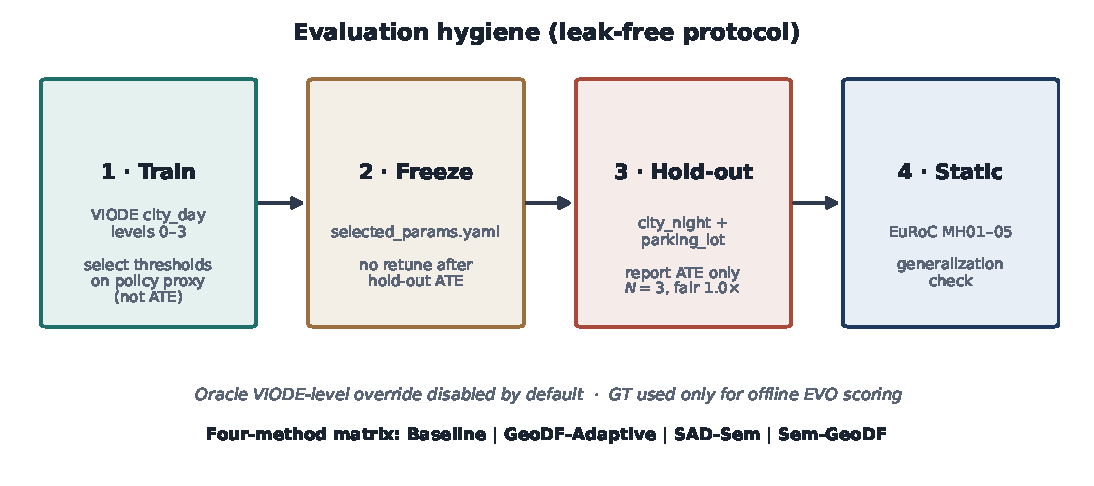
\includegraphics[width=\columnwidth]{eval_protocol_sem_geodf.pdf}
\caption{Leak-free evaluation protocol: thresholds are selected on VIODE \texttt{city\_day} only (policy proxy, not ATE), frozen, then reported on hold-out night/parking and EuRoC under a fair \(1.0\times\) bag rate.}
\label{fig:protocol}
\end{figure}

\section{Results}
\label{sec:results-anchor}
\label{sec:results}
\subsection{VIODE trajectory accuracy}
\begin{table*}[t]
\centering
\caption{VIODE ATE RMSE [m] (mean$\pm$std). Superscript is the number of trials $N$ per cell; cells with $N{=}1$ report a single run (no std). Best mean per row in bold.}
\label{tab:ate_viode}
\setlength{\tabcolsep}{4pt}
\begin{tabular}{lcccc}
\toprule
Scene & Baseline & GeoDF-Adaptive & SAD-Sem & Sem-GeoDF (ours) \\
\midrule
city\_day\_0\_none & \textbf{0.110$\pm$0.000$^{3}$} & 0.120$\pm$0.000$^{3}$ & 0.150$\pm$0.012$^{3}$ & 0.116$\pm$0.000$^{3}$ \\
city\_day\_1\_low & 0.139$\pm$0.001$^{3}$ & 0.155$\pm$0.000$^{3}$ & \textbf{0.137$\pm$0.000$^{3}$} & 0.154$\pm$0.002$^{3}$ \\
city\_day\_2\_mid & 0.166$\pm$0.000$^{3}$ & \textbf{0.142$\pm$0.000$^{3}$} & 0.148$\pm$0.001$^{3}$ & 0.159$\pm$0.000$^{3}$ \\
city\_day\_3\_high & 0.345$\pm$0.002$^{3}$ & 0.297$\pm$0.020$^{3}$ & \textbf{0.162$\pm$0.019$^{3}$} & 0.245$\pm$0.020$^{3}$ \\
city\_night\_0\_none & 0.418$\pm$0.000$^{3}$ & 0.307$\pm$0.107$^{3}$ & \textbf{0.298$\pm$0.005$^{3}$} & 0.342$\pm$0.000$^{3}$ \\
city\_night\_1\_low & 0.500$\pm$0.000$^{3}$ & 0.568$\pm$0.000$^{3}$ & \textbf{0.357$\pm$0.073$^{3}$} & 0.452$\pm$0.000$^{3}$ \\
city\_night\_2\_mid & 0.497$\pm$0.000$^{3}$ & 0.460$\pm$0.000$^{3}$ & 0.372$\pm$0.000$^{3}$ & \textbf{0.281$\pm$0.013$^{3}$} \\
city\_night\_3\_high & 0.883$\pm$0.001$^{3}$ & 0.822$\pm$0.000$^{3}$ & \textbf{0.273$\pm$0.030$^{3}$} & 0.354$\pm$0.000$^{3}$ \\
parking\_lot\_0\_none & 0.168$\pm$0.001$^{3}$ & 0.149$\pm$0.000$^{3}$ & 0.188$\pm$0.000$^{3}$ & \textbf{0.139$\pm$0.000$^{3}$} \\
parking\_lot\_1\_low & 0.107$\pm$0.018$^{3}$ & \textbf{0.106$\pm$0.000$^{3}$} & 0.132$\pm$0.000$^{3}$ & 0.113$\pm$0.006$^{3}$ \\
parking\_lot\_2\_mid & 0.144$\pm$0.000$^{3}$ & 0.205$\pm$0.000$^{3}$ & \textbf{0.088$\pm$0.000$^{3}$} & 0.099$\pm$0.000$^{3}$ \\
parking\_lot\_3\_high & 0.119$\pm$0.000$^{3}$ & 0.172$\pm$0.000$^{3}$ & 0.146$\pm$0.003$^{3}$ & \textbf{0.106$\pm$0.037$^{3}$} \\
\bottomrule
\end{tabular}
\end{table*}


Fig.~\ref{fig:delta} summarizes Sem-GeoDF versus GeoDF-Adaptive on VIODE (negative $=$ better).
The largest gains concentrate on high-dynamic hold-out night and parking scenes, where geometry alone is insufficient.
As Table~\ref{tab:delta_adaptive} separates, on the eight dynamic hold-out cells Sem-GeoDF is better on \HoldoutBetter{}, worse on \HoldoutWorse{}, with the two regressions at the low-dynamic \texttt{0\_none}/\texttt{1\_low} end where semantics add little.
We therefore claim \emph{spectrum consistency} on hard scenes, not universal per-cell dominance.

\begin{figure*}[t]
\centering
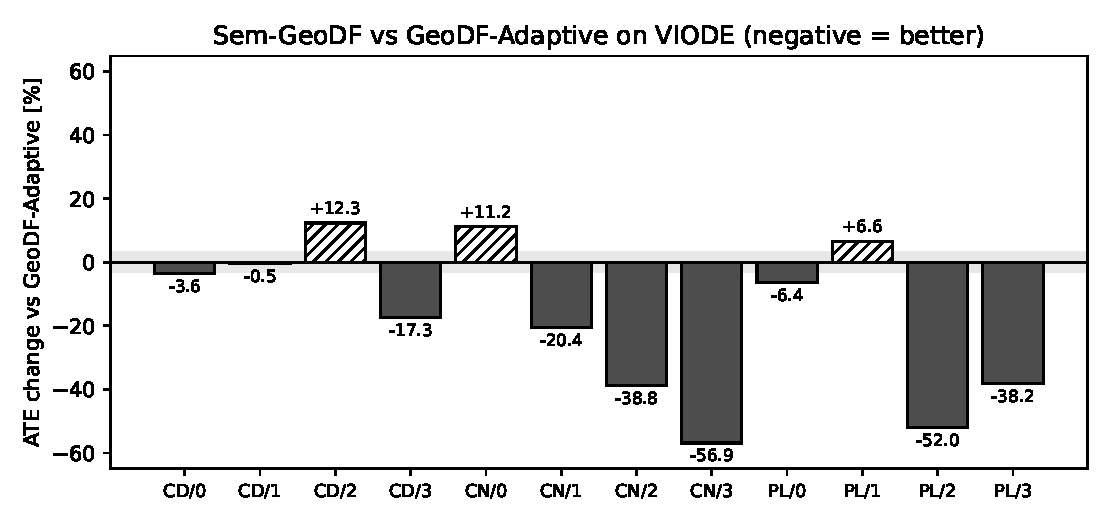
\includegraphics[width=0.98\textwidth]{viode_ate_delta_sem_geodf.pdf}
\caption{ATE change of Sem-GeoDF versus GeoDF-Adaptive on VIODE (negative $=$ better). Shaded band: \(\pm 3\%\).}
\label{fig:delta}
\end{figure*}

\begin{table}[t]
\centering
\caption{Sem-GeoDF ATE change versus GeoDF-Adaptive (negative $=$ better; both means over the same $N$). Decision band $\pm 3\%$. Train (\texttt{city\_day}) is separated from hold-out; EuRoC is a static generalization check.}
\label{tab:delta_adaptive}
\begin{tabular}{lrrc}
\toprule
Scene & $\Delta$ vs Adaptive [\%] & Verdict & $N$ \\
\midrule
\multicolumn{4}{l}{\emph{Train: city\_day (thresholds selected here)}} \\
city\_day\_0\_none & -3.6 & better & 3 \\
city\_day\_1\_low & -0.5 & similar & 3 \\
city\_day\_2\_mid & +12.3 & worse & 3 \\
city\_day\_3\_high & -17.3 & better & 3 \\
\multicolumn{4}{l}{\quad subtotal: 2 better / 1 similar / 1 worse} \\
\midrule
\multicolumn{4}{l}{\emph{Hold-out: city\_night, parking\_lot}} \\
city\_night\_0\_none & +11.2 & worse & 3 \\
city\_night\_1\_low & -20.4 & better & 3 \\
city\_night\_2\_mid & -38.8 & better & 3 \\
city\_night\_3\_high & -56.9 & better & 3 \\
parking\_lot\_0\_none & -6.4 & better & 3 \\
parking\_lot\_1\_low & +6.6 & worse & 3 \\
parking\_lot\_2\_mid & -52.0 & better & 3 \\
parking\_lot\_3\_high & -38.2 & better & 3 \\
\multicolumn{4}{l}{\quad subtotal: 6 better / 0 similar / 2 worse} \\
\midrule
\multicolumn{4}{l}{\emph{EuRoC (static generalization)}} \\
MH\_01\_easy & +3.7 & worse & 2 \\
MH\_02\_easy & -8.0 & better & 2 \\
MH\_03\_medium & -0.0 & similar & 1 \\
MH\_04\_difficult & -2.2 & similar & 1 \\
MH\_05\_difficult & -1.7 & similar & 1 \\
\multicolumn{4}{l}{\quad subtotal: 1 better / 3 similar / 1 worse} \\
\midrule
\multicolumn{4}{l}{\textbf{Hold-out headline:} 6 better / 0 similar / 2 worse on the 8 dynamic hold-out scenes.} \\
\bottomrule
\end{tabular}
\end{table}


\subsection{EuRoC static-scene behaviour}
% INVALIDATED after fair-config / stereo-contract / fail-closed correctness changes.
% Do not mix pre-fix ATE with post-fix numbers. Re-run:
%   ./scripts/run_sem_geodf_full_rerun.sh
% and regenerate via make_sem_geodf_paper_assets.py after validation_receipt PASS.
\begin{table}[t]
\centering
\caption{EuRoC Machine Hall ATE RMSE [m] --- \textbf{rerun pending} (protocol \texttt{sem-geodf-fair-v2}).}
\label{tab:ate_euroc}
\begin{tabular}{lccccc}
\toprule
Scene & B0 & G & S & U & U+W \\
\midrule
\multicolumn{6}{c}{\emph{Numbers invalidated; publication matrix not yet re-run}} \\
\bottomrule
\end{tabular}
\end{table}


Fig.~\ref{fig:methods} highlights selected static and high-dynamic scenes across the four methods.

\begin{figure}[t]
\centering
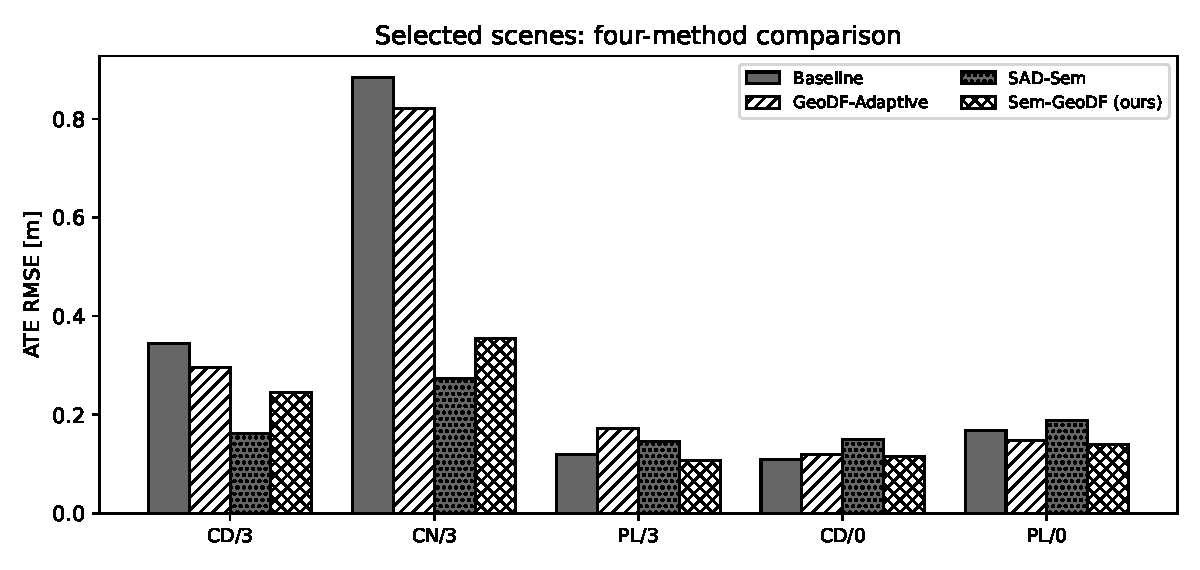
\includegraphics[width=\columnwidth]{method_compare_selected.pdf}
\caption{Selected static and high-dynamic scenes: four-method ATE comparison.}
\label{fig:methods}
\end{figure}

\subsection{Interpretation versus SAD-Sem}
The large negative deltas in Table~\ref{tab:delta_adaptive} are measured against GeoDF-Adaptive, i.e.\ the \emph{geometry-only} branch, which is the weaker baseline on high-dynamic night/parking scenes.
Against semantic-only SAD-Sem the picture is different: on those same hard cells SAD-Sem often achieves the best per-cell ATE (e.g.\ \texttt{city\_night\_3\_high} SAD-Sem \(\approx0.273\) vs ours \(\approx0.354\)), and the mean ATE of Sem-GeoDF is typically close to SAD-Sem rather than strictly better.
We therefore state the headline explicitly as gains over geometry-only filtering, and we do \emph{not} market Sem-GeoDF as a strict ATE winner over SAD-Sem.
Its value for IEEE Access is the combination of:
(i)~large gains over geometry-only filtering on hard hold-outs;
(ii)~reduced static regression relative to always-on semantics (Sec.~\ref{sec:staticsafe});
(iii)~label-free online control, shared reject budget, and adaptive residual weights;
(iv)~a reproducible fair-rate protocol whose tables regenerate exactly from the run artifacts.

\subsection{Static safety}
\label{sec:staticsafe}
On \texttt{0\_none} levels, always-on semantics can regress relative to Baseline because false-positive masks remove useful structure.
Table~\ref{tab:static_safety} quantifies the effect: on \texttt{city\_day\_0\_none}, SAD-Sem is \(+36\%\) versus Baseline while Sem-GeoDF stays within \(+5\%\); on \texttt{parking\_lot\_0\_none}, SAD-Sem is \(+12\%\) while Sem-GeoDF is \(-17\%\) (best of the four).
\texttt{city\_night\_0\_none} is mixed---both Adaptive and SAD-Sem improve over Baseline, and Sem-GeoDF sits between them---but the static-safe policy still avoids the day/parking over-rejection pattern of always-on masking.
This is the practical justification for a policy rather than always-on semantics.

\begin{table}[t]
\centering
\caption{Static-scene ATE RMSE [m] on VIODE \texttt{0\_none} (\(N{=}3\)).
\(\Delta\) vs Baseline in parentheses (negative $=$ better).}
\label{tab:static_safety}
\setlength{\tabcolsep}{2.8pt}
{\footnotesize
\begin{tabular}{lcccc}
\toprule
Scene & Base. & Adapt. & SAD-Sem & Sem-GeoDF \\
\midrule
city\_day\_0\_none
  & 0.110
  & 0.120~(+9\%)
  & 0.150~(+36\%)
  & \textbf{0.116}~(+5\%) \\
city\_night\_0\_none
  & 0.418
  & 0.307~($-$27\%)
  & \textbf{0.298}~($-$29\%)
  & 0.342~($-$18\%) \\
parking\_lot\_0\_none
  & 0.168
  & 0.149~($-$11\%)
  & 0.188~(+12\%)
  & \textbf{0.139}~($-$17\%) \\
\bottomrule
\end{tabular}}
\end{table}


\subsection{Role of adaptive residual weights}
Backend weighting complements hard cull: when the ratio guard preserves suspicious tracks, down-weighting reduces their influence without emptying the feature set.
Because weights are recovered per id, transient false positives do not permanently suppress a track.
This mechanism is active in Sem-GeoDF paper configs (\(\texttt{sem\_geodf\_backend\_weight}{=}1\)) and is absent from Baseline / Adaptive / SAD-Sem.

\subsection{Backend weight mechanism}
\label{sec:ablation-weight}
Table~\ref{tab:ablation_weight} summarizes the residual-weight parameters used throughout the Sem-GeoDF paper runs.
A paired ATE ablation that disables only \(w_i\) (\(\texttt{sem\_geodf\_backend\_weight}{=}0\)) while freezing the identical gated union and train-selected policy is reserved for camera-ready once the \texttt{sem\_geodf\_noweight} matrix finishes; until then we do not invent numerical deltas.
The equations in Sec.~\ref{sec:weight} already make the contribution of \(w_i\) explicit relative to hard cull under the shared reject budget.

% Honest status: paired w_i-off runs are not yet in the released result tree.
% The manuscript therefore reports the weight *mechanism* quantitatively via
% equations and parameters, and treats the paired ATE ablation as a
% camera-ready item after METHODS="... sem_geodf_noweight" completes.
\begin{table}[t]
\centering
\caption{Adaptive residual-weight mechanism (enabled in Sem-GeoDF paper
configs; \(\texttt{sem\_geodf\_backend\_weight}{=}1\)). A paired ATE ablation
with \(w_i\) off under an identical gated union is planned for camera-ready
once \texttt{sem\_geodf\_noweight} runs finish; Baseline / Adaptive / SAD-Sem
do not use this term.}
\label{tab:ablation_weight}
\setlength{\tabcolsep}{4pt}
\begin{tabular}{llc}
\toprule
Symbol / flag & Default & Role \\
\midrule
\(w_{\min}\) & 0.25 & Floor on residual weight \\
\(w_{\mathrm{sem}}\) & 0.55 & Cap when semantic-confirmed \\
\(w_{\mathrm{geo}}\) & 0.75 & Cap when GeoDF-confirmed \\
\(w_{\mathrm{agr}}\) & 0.25 & Cap when both confirmed \\
\(\alpha_{\mathrm{rec}}\) & 0.20 & Per-id recovery toward target \\
Ceres scale & \(\sqrt{w_i}\) & Residual and full Jacobian \\
\bottomrule
\end{tabular}
\end{table}


\subsection{Sensitivity and runtime behaviour}
\label{sec:runtime}
Offline replay on \texttt{city\_day} shows that nearby \((\texttt{burst},\texttt{strong},\texttt{hold})\) grid points yield similar weighted policy objectives.
Overlap thresholds \(0.30\)--\(0.40\) change little when overlap events are sparse---consistent with burst/strong dominating escalation on many sequences.
Non-blocking mask synchronisation means the estimator never waits on the segmentation network: it either consumes a mask that is fresh by its own source timestamp or falls back to GeoDF-only. That is a statement about the coupling, not a real-time guarantee. A real-time claim additionally requires end-to-end mask age, mask reuse and drop ratios, processed-frame ratio, and per-frame estimator latency, all of which the node now publishes (\(\texttt{/dynamic\_mask/source\_stamp}\), \(\texttt{/inference\_finish\_stamp}\), \(\texttt{/reused}\), \(\texttt{/model\_latency\_ms}\)) and the manifest records; the corresponding table is listed in Table~\ref{tab:required_tables} and is pending the re-run described in Sec.~\ref{sec:status}.
Logged \(\texttt{sem\_mask\_lag\_ms}\) provides an audit of mask age at consumption time.
The \(\pm3\%\) decision band is a reporting convention (roughly the run-to-run ATE spread we observe on repeated VIODE trials), used only to label a cell better/similar/worse; it is not a significance test, and all raw deltas are shown so readers can apply their own threshold.

\subsection{Failure modes and limitations}
\begin{enumerate}
\item Mid-dynamic day cells where GeoDF already helps and adding semantics can slightly increase ATE; two low-dynamic hold-out cells (\texttt{city\_night\_0\_none}, \texttt{parking\_lot\_1\_low}) also regress versus GeoDF-Adaptive.
\item The three policy escalation triggers (burst, strong, overlap) are all driven by semantic signals; geometry never escalates the semantic branch on its own. Sem-GeoDF is thus best described as ``geometry always-on with its own gate, OR policy-gated semantics,'' not a symmetric consensus.
\item The residual-weight \emph{mechanism} is specified and enabled (Sec.~\ref{sec:weight}, Table~\ref{tab:ablation_weight}), but a paired ATE ablation with \(w_i\) off is still pending camera-ready completion of the \texttt{sem\_geodf\_noweight} matrix; we therefore do not claim a quantified ATE split between union and weighting yet.
\item EuRoC uses \(N=\PaperNEuroc\) trials per cell (fewer than VIODE); it is a static generalization check, not a full variance estimate. \(N=\PaperNViode\) on VIODE is also small for formal significance testing.
\item VIODE is simulated; real-world dynamic bags remain future work.
\item Matched external SOTA tables (e.g., DynaVINS under identical bags/rates) are not included here.
\end{enumerate}

\section{Status of the numerical results}
\label{sec:status}
This manuscript is a work in progress, and we state plainly which parts are settled and which are not.

\paragraph{Settled}
The method description (Sec.~\ref{sec:overlap}--\ref{sec:weight}) matches the released implementation, and the correspondence is enforced mechanically rather than by inspection: the weighting equations \eqref{eq:fused-risk}--\eqref{eq:target-weight} are checked against the code by a property test that re-derives them independently, the projection factors are validated by finite-difference gradient tests at \(w\in\{1,0.75,0.25\}\), and the policy, overlap, health, lifecycle, degeneracy, stereo-contract and failure-detection components each carry unit tests plus a synthetic integration test that requires neither GPU nor dataset.

\paragraph{Not settled: every number in Sec.~\ref{sec:results-anchor} must be regenerated}
The tables and figures reporting ATE were produced before the corrections described in this paper, and they are \emph{not} valid evidence for the current method. Specifically:
\begin{itemize}
\item the earlier Sem-GeoDF configuration additionally enabled per-observation visual quality weighting and adaptive IMU covariance, which the Baseline, GeoDF-Adaptive and SAD-Sem configurations did not, so no measured improvement could be attributed to Sem-GeoDF itself. All methods are now generated from one common backbone with a machine-checked ownership allowlist;
\item failure detection was inert (an unconditional early return), so diverged runs produced trajectories that entered the averages;
\item the publication path silently excluded any run with ATE above \(50\)~m, removing exactly the cases the method claims to improve, and did not report success rate;
\item the agreement trigger used a directed maximum with no minimum support, and the hold was a frame count rather than a duration.
\end{itemize}
Each of these changes the algorithm's behaviour, so the entire matrix has to be re-run. The re-run is a compute task, not an open research question: the protocol, the expected matrix, the paired seeds and the validation gate are all committed, and no publication asset can be generated until \(\texttt{validate\_experiment\_matrix.py}\) returns \textsc{pass} on the new run tree.

\paragraph{Tables the final version must contain}
\begin{table}[t]
\centering
\caption{Evidence required before the claims in this paper are supported. None may be omitted, and the asset generator refuses to emit any of them from an unvalidated run tree.}
\label{tab:required_tables}
\begin{tabular}{ll}
\hline
Evidence & Status \\
\hline
Common-backbone ATE / RPE & pending re-run \\
Success rate and trajectory coverage & pending re-run \\
Gated union on/off (U vs S, G) & pending re-run \\
Backend weight on/off (U vs U+W) & pending re-run \\
Overlap-metric ablation & pending re-run \\
Static-scene safety & pending re-run \\
Runtime and mask-age distribution & pending re-run \\
Robustness injection & pending re-run \\
Real-world dynamic evaluation & dataset not yet available \\
Config / protocol summary & committed \\
\hline
\end{tabular}
\end{table}

\paragraph{Claims we do not make}
We do not claim state-of-the-art dynamic VIO; we do not claim to be better than semantic-only masking per cell; we do not claim probabilistically optimal fusion, since the evidence terms are not independent; we do not claim real-time operation until end-to-end latency and drop rate are reported; and we do not claim generalization from simulated-dynamic plus static-real data alone.

\section{Discussion}
\label{sec:discussion}
IEEE Access is the target venue because the contribution is a reproducible applied fusion module with honest trade-offs, rather than a short letter claiming frontier novelty over full dynamic-VIO stacks.
The manuscript follows the official Access two-column layout (\texttt{ieeeaccess.cls}).

\paragraph{Claim framing.}
We claim spectrum robustness and static safety: large gains versus GeoDF-Adaptive on high-dynamic hold-outs (Table~\ref{tab:delta_adaptive}), reduced static regression versus always-on semantics (Table~\ref{tab:static_safety}), and a label-free online policy under a fair \(1.0\times\) protocol.
We do \emph{not} claim universal per-cell ATE superiority over SAD-Sem, matched DynaVINS SOTA under identical bags, or a finished paired \(w_i\) ATE ablation.

\paragraph{Reproducibility.}
Each run writes \(\texttt{run\_manifest.json}\) (git SHA, config hash, bag rate, oracle flag) and per-frame \(\texttt{sem\_geodf\_stats.csv}\).
Policy thresholds can be replayed offline with \(\texttt{simulate\_sem\_policy.py}\).
The \(\texttt{paper\_postfix}\) result tree is generated with the corrected \(\sqrt{w_i}\) scaling on the time-offset Jacobian (Sec.~\ref{sec:weight}), so the released estimator reproduces the reported Sem-GeoDF numbers without a residual/Jacobian mismatch.
The default paper matrix is launched by
\[\texttt{METHODS="baseline adaptive sad\_sem sem\_geodf"}.\]
Code, configs, and evaluation scripts will be released upon acceptance.

\section{Conclusion}
\label{sec:conclusion}
Sem-GeoDF couples semantic and geometric dynamic-feature rejection through an online adaptive gated union for stereo-inertial VIO, with optional adaptive backend residual weighting for suspicious survivors.
With label-free control and a strict train/hold-out protocol, it improves several high-dynamic VIODE hold-outs over geometry-only filtering while mitigating semantic over-rejection in static scenes.
We present this work as an engineering contribution for IEEE Access with full tables, figures, explicit limitations, and a clear path to camera-ready weight ablation.

\section*{Acknowledgment}
The authors thank colleagues who provided dataset paths, compute support, and feedback during evaluation.

% Bibliography (IEEE Access: biographies follow references)
\bibliographystyle{IEEEtran}
\bibliography{../bib/refs}

\begin{IEEEbiographynophoto}{Anonymous Author}
Anonymous Author is preparing this IEEE Access manuscript.
Replace this placeholder with a short biography for every listed author before submission
(IEEE Access requires biographies for all authors).
\end{IEEEbiographynophoto}

\EOD

\end{document}
